\section{Introduction}

Since the rise of atomic clocks, the precise progression of time is measured by
examining the radioactive decay of atoms. In computing, this is often simulated
by quartz clocks that trade a lower accuracy for affordability in everyday
technology. To enable the use of time in human communication, standards like
\ac{UTC} define the precise time at a given moment as points of reference.
However, what is colloquially called \emph{wall-clock time} is an inherently
human-made concept that is agreed upon by social convention. Unix systems, for
example, translate \ac{UTC} to \emph{system time} as the number of passed
seconds since the 1st of January 1970. As such, wall clock time in computing is
a challenging task that is nowadays dealt with by utilizing time servers and
running time synchronization protocols.

In the area of secure systems, recent years have seen the rise of capable
confidential computing solutions that can protect data in use, such as Intel
SGX, AMD SEV, Intel TDX, and ARM CCA. The key idea behind these \acp{TEE} is to
protect critical code and data in so-called \emph{enclaves} that are isolated
from the rest of the system stack. Particularly, while the privileged operating
system and hypervisor remain in charge of enclave resource management and
availability, any direct access to enclave code or data is prevented by means of
hardware-level access control logic. \acp{TEE} can, hence, effectively protect
sensitive data while it resides in memory. However, enclaves may still request
untrusted network communication from the potentially hostile operating system to
perform computations.

The challenge of time-keeping in the context of confidential computing can be
troubling in multiple ways. First, agreeing on time in a distributed context
often relies on external trusted time servers, together with an approximation of
the time delay between server and recipient. However, enclaves that need time
information have to to communicate with remote servers through an untrusted,
attacker controlled environment. This potentially allows the adversary to
unpredictably delay network packets. Second, even if no trusted time server is
utilized and time is only communicated between local peers, adversaries can
often control the execution and interruption of enclaves, which may give the
attacker some control to induce further delays.

In this paper, we investigate the challenge of reasoning about time and
providing temporal guarantees in the context of confidential computing.
Particularly, we identify five levels of increasingly more capable time tracking
approaches and overview existing timing capabilities in popular TEEs, with an
explicit focus on the widespread Intel SGX architecture and software ecosystem.
Our specific contributions are:
\begin{itemize}
	\item We identify five distinct levels of tracking the passage of time from
	within isolated enclaves.
	\item Focusing on Intel SGX, we analyze which time levels can be provided
	to enclaves and how this is used by the software ecosystem and in selected
	academic work.
 	\item We classify other TEE architectures and analyze their limitations in
 	regards to trusted time-keeping.
 	\item Lastly, we overview use cases and applications, highlighting the
 	overall difficulty of guaranteeing trusted time in untrusted environments.
\end{itemize}

\section{System Model}

We consider a general \ac{TEE} architecture, where a security-critical
application executes in a trusted enclave protection domain that is isolated
from any other software on the system, including the privileged operating system
and hypervisor. The enclave may further include a shielding system that offers
trusted services to the application, e.g., in form of a library OS or \ac{SDK}.

This study considers applications that need some notion of ``wall-clock time''
from a trusted time source in order to realize their security objectives. The
time source could be local, e.g., a secure timestamp counter in the CPU, or
remote, e.g., a trusted server. We explicitly focus on reasoning about the
wall-clock time that passes between two execution points, which does not
necessarily correspond to the actual running time of the enclave. That is, while
the latter may be easier to measure, e.g., by counting the number of
instructions executed in the enclave, it is decidedly {not} a good proxy for
wall-clock time in the presence of attacker-induced interrupts that may
arbitrarily delay enclave execution.

Note that in case the application needs \emph{absolute} wall-clock time, i.e.,
calendar time, an extra step may be needed such as an initial time
synchronization with a trusted source.

\section{Notions of Time}
\label{section:notions-time}
\newcommand{\Tzero} {T\textsubscript{0}\xspace}
\newcommand{\Tone}  {T\textsubscript{1}\xspace}
\newcommand{\Ttwo}  {T\textsubscript{2}\xspace}
\newcommand{\Tthree}{T\textsubscript{3}\xspace}
\newcommand{\Tfour} {T\textsubscript{4}\xspace}

\sclist{0.6}{%
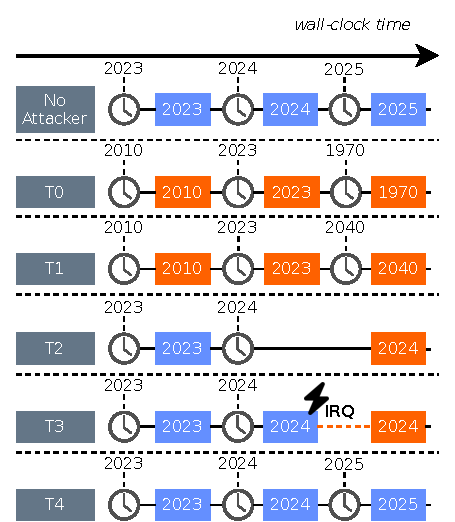
\includegraphics{figures/time-levels.pdf}}{Visual representation of different time levels}%
  {Visual representation of different time levels with attacker
  influences marked in orange. \Tzero{} is controlled by the attacker, \Tone can
  only move forward but make jumps, \Ttwo can be arbitrarily delayed, and
  finally in \Tthree the attacker can still interrupt the enclave before it
  utilizes the time. Instead, level \Tfour{} gives the same guarantees as when
  no attacker is present.}%
  {fig:time-types} 

\newcolumntype{Y}{>{\centering\arraybackslash}X}
\begin{sidewaystable}
	\renewcommand{\tableNo}{}
	\renewcommand{\tableYes}{\faCheck}
	%\renewcommand{\arraystretch}{2}
	\setlength{\extrarowheight}{10pt}
	\centering
	\footnotesize
    \begin{tabularx}{\textwidth}{llccccXX}    \toprule
        % \bf Type 	& \bf Added guarantee 	& \multicolumn{4}{c}{\bf Attacker controls\dots} & \bf Example time sources &  \bf Discussed use case\\
        % \cmidrule(lr){3-6}
			Type		&	Added guarantee				        & Rollback & Freq. & Delay & Interrupt & Example time source & Discussed use case \\ 
			\midrule
			\Tzero  & None   							          & \tableNo & \tableNo & \tableNo & \tableNo & Untrusted OS    				& ---       \\
			\Tone   & Time monotonically advances   & \tableYes & \tableNo & \tableNo & \tableNo & Untrusted OS \texttt{+} check & Time-based policies        \\
			\Ttwo   & Time moves at constant pace   & \tableYes & \tableYes & \tableNo & \tableNo & ME, timer thread, remote server			& Rate limiting       \\
			\Tthree & Time is read with known delay & \tableYes & \tableYes & \tableYes & \tableNo & Secure TSC, MMIO timer	& Resource counting      \\
			\Tfour  & Use of time is atomic  			  & \tableYes & \tableYes & \tableYes & \tableYes & Trusted scheduler & Credential expiration, DRM       \\
			\bottomrule
		\end{tabularx}
	\caption[Levels of time and the guarantees given by them]{
		Levels of time and the guarantees given by them. Checkmarks identify that a level protects against this type of attack.
	}
	\label{tab:time-types}
	% \vspace{-2ex}
\end{sidewaystable}

This section identifies five successive levels of time tracking approaches for
confidential applications, summarized in \cref{tab:time-types}. These levels are
additive, so that each level represents an increasingly more capable and
accurate time source. However, higher levels may also place more demands on the
underlying TEE architecture, and, as discussed later, lower levels may be
sufficient for certain applications.

\Cref{fig:time-types} depicts each time level, together with a sample time trace
reported to and experienced by the enclave. The top row represents the ground
truth, where no attacker is present and wall-clock time advances linearly and at
a constant rate. The running time of the enclave application is visualized in
the colored squares, whereas the clock symbols represent a query to the abstract
time source. The example value returned by the time source is indicated above
the clock symbol and will be used in the subsequent enclave computation, colored
blue if the time is correct w.r.t.\ the wall-clock time, or orange if time is
influenced by the attacker.

\paragraph{\Tzero: No trusted time}
The default case is to have no trusted time, i.e., to fully rely on untrusted
input without performing any checks on the incoming time data. As illustrated in
\cref{fig:time-types}, the observed time can be any point in the past or in the
future and may vary arbitrarily. While this may suffice for testing scenarios,
e.g., annotating untrusted timestamps in a debug log, it is clear that any
application-specific, security-sensitive use of time cannot rely on a \Tzero{}
timer.

\paragraph{\Tone: Monotonically increasing time}
If enclaves only have access to an untrusted time source, they can perform
certain minimal checks on received timestamps before acceptance. The most
important check to perform here is to ensure that received time data only ever
increases, i.e., that time never winds backwards. Depending on the granularity
of the untrusted time source and the sampling frequency, additional checks may
be added, e.g., checking that two time queries should never return the same
value or zero. While these checks are minimal and the underlying time source is
still untrusted, the counter value can be stored inside the enclave and \Tone{}
can at least prevent attackers from rewinding  the internal time of an enclave.
Since \Tone{} timers cannot rely on external data, they have to store the time
locally. This makes them prone to rollback attacks where time is reverted by
restarting the enclave with an obsolete local timestamp.

\cref{fig:time-types} shows that attackers in \Tone{} can advance time at will
and can trigger arbitrarily large time jumps for the enclave.

\paragraph{\Ttwo: Trusted remote time}
To improve time-keeping, the enclave can switch from an untrusted to a remote
trusted time source, guaranteed to have a fixed, known frequency. As such, this
time source can be relied upon for trusted time information, when standard
cryptographic measures are in place to protect and validate the integrity and
authenticity of the time packets over the untrusted network (e.g., this secure
time channel can be configured as part of the attestation protocol). Note that
the ``remote'' trusted time source can be truly remote, e.g., a server reached
over the Internet, but could also be provided on the same system-on-chip, e.g.,
by a trusted co-processor. If the monotonicity of the external time source can
be trusted, rollback attacks targeting the time value are also not possible
anymore since on enclave restarts, the time can be re-queried. Obviously,
rollback attacks are still a threat to enclaves with a \Ttwo{} timer and above,
but they will not affect the time stored in the enclave.

As the communication channel between the time source and the enclave is still
under the attacker's control in regards to availability, \Ttwo{} time requests
and responses may be arbitrarily delayed. Hence, \Ttwo{} timestamps received by
the enclave can only ever be trusted as a \emph{lower bound} on the reference
wall-clock time. \Cref{fig:time-types} depicts a potential situation where the
attacker would allow the enclave to query the time source, but then delay the
response.

\paragraph{\Tthree: Trusted local time}
In order to prevent arbitrary delay attacks, enclaves must be able to access the
trusted time source through a direct channel without adversary intervention,
e.g., when the time source is an on-chip timestamp counter that can be queried
via dedicated CPU instructions. If both time source and channel are trusted,
adversaries cannot arbitrarily delay timestamps anymore before they reach the
enclave. This, technically, grants enclaves access to accurate time information
with both a lower and an \emph{upper bound}.

We argue, however, that in order to utilize such accurate time information in
practice, enclaves also need to be able to act \emph{atomically}, i.e., without
(undetected) attacker-induced interruptions. \Cref{fig:time-types} depicts a
possible attack that is still possible on \Tthree where the adversary precisely
interrupts the enclave right after it reads from the trusted time source. The
adversary can then keep the enclave interrupted until it suits them and only
resume the enclave at a convenient time, effectively reducing the accurate
temporal guarantees back to only the lower bound offered by a \Ttwo time source.

Consider an enclave that only grants access to a resource if a presented
certificate is valid, and denies access otherwise. If the adversary begins the
validation process at a time that the certificate is still valid, the enclave
will read a permissible time from the time source. Right after the time value
has been read into the enclave, the adversary could however interrupt the
enclave. When the enclave is later resumed, the adversary could gain access to
the resource even if the initially presented certificate is not valid anymore.

\paragraph{\Tfour: Trusted and atomic local time}
The dangers of the above attack vector are nuanced. Many interruption attacks on
\Tthree timers only work if the adversary initially had access to a resource.
Thus, arguably, maintaining this access until after the credentials expired can
be considered as a parallel issue to denial of service attacks where output of
the enclave is delayed by the adversary. We note, however, that for some
applications and use cases this attack vector may not be acceptable and enclaves
should only present an output at the correct time. We discuss two examples of
this in \cref{sec:usecases:tfour}.

\section{Intel SGX}
\label{arch:sgx}

The Intel SGX architecture does, in itself, not provide any notion of trusted
time. However, several proposals exist to provide trusted time services to SGX
enclaves.

\paragraph{Platform service}
Intel provides \ac{PSW} to set up and use trusted time and monotonic
counters~\cite{cen2017trusted}. Particularly, the PSW offers a \Ttwo{} time
source based on a coarse-grained clock in the Intel \ac{ME}, a chip that
physically resides on the same package but is entirely separate from the main
CPU. This allows timer-based policy enforcements on offline platforms that are
not necessarily connected to a network. All communication between enclaves and
the \ac{ME} passes via the untrusted operating system and is, hence,
cryptographically protected, but can be arbitrarily delayed. Enclaves can use
the \texttt{sgx\_get\_trusted\_time} API to track the amount of time (in
seconds) passed since a previous read of the timer. ME services are excluded in
the Intel SGX Linux PSW from version 2.8 from 2020 onwards.

\paragraph{Timestamp counter}
Initial SGX versions did not allow to execute the x86 \inst{RDTSC} instruction
to receive the processor's internal \ac{TSC} in enclaves. However, more recent
SGX2 processors now support the \inst{RDTSC} instruction in enclave mode, with
an explicit warning that the instruction may be trapped and the timestamp
returned may be influenced by the untrusted operating system.

We experimentally confirmed that privileged adversaries can arbitrarily control
the values returned by \inst{rdtsc} on SGX2 platforms by directly manipulating
the underlying \texttt{IA32\_TIME\_STAMP\_COUNTER} \ac{MSR}. For this, we
developed a sample enclave that executes two \texttt{rdtsc} instructions and
returns the measured cycle difference. One would expect this difference to
always be positive and reflect the elapsed time in between the two \inst{rdtsc}
instructions. However, in our proof-of-concept, we make the observed time in the
enclave move ``backwards'' by interrupting the enclave and overwriting the
\ac{TSC} value using the privileged \inst{wrmsr} instruction in between both
\inst{rdtsc} calls. Thus, we conclude that \inst{rdtsc} on current SGX platforms
is not any better than an adversary-controlled \Tzero{} timer.

We note, however, that the \ac{TSC} \ac{MSR} is duplicated per logical processor
and can, hence, only be changed by interrupting the enclave. That is, as long as
the enclave is not interrupted, any successive \inst{rdtsc} reads will behave as
a trusted \Tfour{} timer that monotonically increases at fixed frequency. This
may be leveraged with upcoming ISA changes~\cite{intel2022aexnotify} that will
make SGX enclaves interrupt-aware. At the same time, the restriction that an
enclave is never interrupted may be too limiting for some real-world
deployments.

\paragraph{Academic timers}

TrustedClock~\cite{jigsaw} is a system that relies on an interrupt handler in
\ac{SMM} to implement functionality that is similar in its security guarantees
to \texttt{sgx\_get\_trusted\_time} by the Intel SGX \ac{PSW}. The authors base
their security argument on the handler being loaded at boot time with a secret
key that is not accessible at runtime by the untrusted OS. Enclaves can then
communicate with the handler by establishing a secure channel based on the
pre-shared public key. Aside from the security implications of including the
unattested SMM handler in the trusted computing base, TrustedClock is stated to
not be completely immune to timer modifications by the untrusted OS. Instead,
TrustedClock relies on combining several x86 hardware timers and asserting their
monotonicity (similar to \Tone{}), thus making it harder for a malicious OS to
precisely tamper with all involved timers at the same time.

TimeSeal~\cite{anwar2019securing} utilizes a cohort of multiple threads that
each periodically poll \texttt{sgx\_get\_trusted\_time} to monotonically
increase the time. The authors argue that by using multiple threads and nuanced
synchronization policies between the threads, attacks can be limited in their
scope. Nonetheless, attackers that delay or prevent scheduling of timer threads
at convenient times, such as right before a thread returns a time response, will
be able to skew the reported time of TimeSeal. Additionally, with the
discontinuation of \texttt{sgx\_get\_trusted\_time} on Linux systems, TimeSeal
may not be implementable anymore as of today.

%\newcommand{\xrot}[1]{\hspace{-.4em}\rotatebox{20}{\footnotesize#1}\hspace{-.4em}}
\newcommand{\xrot}[1]{#1}
\newcommand{\xtwo}{\Ttwo{}}
\newcommand{\xone}{\Tone{}}
\newcommand{\xzero}{\Tzero{}}
\newcommand{\xpoc}{\Tzero{}*}
\newcommand{\xna}{--}
\newcommand{\xcat}[2]{\multirow{#1}{*}{\rotatebox{90}{\footnotesize\textsl{#2}}}}
\begin{table}[t]
  %\vspace{-1ex}
  \centering
  %\vspace{-2ex}
  \adjustbox{max width=\linewidth}{
  \setlength\tabcolsep{3pt}  
  \begin{tabular}{ccccccccc}
  \toprule
  \xrot{SDK} & \xrot{OE} & \xrot{EDP} & \xrot{Gramine} & \xrot{LKL} & \xrot{Occlum} & \xrot{Mystikos} & \xrot{Ego} & \xrot{Enarx} \\
  \midrule
  \href{https://github.com/intel/linux-sgx/releases/tag/sgx_2.8}{---}/\href{https://cdrdv2-public.intel.com/671508/sgx-sdk-developer-reference-for-windows-os.pdf}{\xtwo} & 
  \href{https://github.com/openenclave/openenclave/blob/cd72fd7069488ba6f453c8f5f47bd9fd9a6e6c0d/enclave/core/time.c#L8}{\xpoc} & 
  \href{https://github.com/fortanix/rust-sgx/blob/a7ee253352856b35e54be22c505775c6556ffa82/intel-sgx/enclave-runner/src/usercalls/mod.rs#L1555}{\xzero} & 
  \href{https://github.com/gramineproject/gramine/issues/595}{\xone} & 
  \href{https://github.com/lsds/sgx-lkl/blob/b6e838e0034de86b48470b6a6bf87d2e262e65c9/src/enclave/enclave_timer.c#L29}{\xone} & 
  \href{https://github.com/occlum/occlum/blob/500ca21d527f700d458df10b891948627f396d97/src/libos/src/time/mod.rs#L76}{\xpoc} & 
  \href{https://github.com/deislabs/mystikos/blob/7ce616416a310aabb543517ed3a9625c1f4acb70/kernel/itimer.c#L32}{\xzero} & 
  \href{https://github.com/edgelesssys/edgelessrt/blob/9191ff25a0424d21a22c85eb12b09ebe5f407c3f/src/ertlibc/time.cpp#L53}{\xone} & 
  \href{https://github.com/enarx/enarx/blob/4c1d3db4039e1f2af4b251a202e64a2cdc0729fb/crates/sallyport/src/guest/call/syscall/clock_gettime.rs#L16}{\xzero} \\
  \bottomrule
\end{tabular}
}
\caption[Intel SGX software projects and their use of time]{Intel SGX software projects and their use of time. Stars indicate that we prototyped a proof of concept to roll back time for a project. Intel SDK is shown for Linux/Win.
}
\label{tab:sgx-overview}
% \vspace{-2ex}
\end{table}

\paragraph{Software ecosystem}
Several shielding systems offer a ``lift-and-shift'' approach to port legacy
applications to SGX. However, these applications were not designed for SGX's
threat model and may rely on sane OS time services.

\Cref{tab:sgx-overview} summarizes how existing SGX shielding systems expose the
untrusted OS time to applications. Interestingly, we found that most projects
include a warning, but forward OS time without any restrictions (\Tzero{}),
whereas the Gramine and LKL library operating systems at least ensure that time
does not move backwards (\Tone{}). We developed two minimal proof-of-concepts to
demonstrate backwards time advances in OpenEnclave and Occlum. We, hence,
recommend that all projects include minimal checks to adopt the \Tone{} time
model.

\section{Other Architectures}
\paragraph{Intel TDX}

The TDX specification~\cite{intelTdxSpec} discusses \ac{TSC} virtualization,
which provides a consistent virtual \ac{TSC} value to a \ac{TD} among all its
vCPUs. The virtual \ac{TSC} starts counting from zero when the \ac{TD} is
initialized and runs at a fixed frequency defined by a parameter stored in the
TD configuration. Guest \acp{TD} can access the virtual \ac{TSC} using the
\inst{RDTSC} instructions, and its value is calculated from the physical
\ac{TSC} adjusted to the \ac{TD}'s offset and frequency. 

We analyzed the source code of the TDX module, which makes sure that the
\ac{TSC} is not modified before a \ac{TD} enter by comparing the current
\texttt{TSC\_ADJUST} \ac{MSR} value against a reference value stored on \ac{TD}
creation, raising an exception if a mismatch between the two values occurs. This
allows \acp{TD} to obtain a stable and consistent \ac{TSC} value across \ac{TD}
lifetime, guaranteeing a time level \Tthree{}.

\paragraph{AMD SEV}

The AMD SEV-SNP~\cite{AmdSevSnp} extensions introduced a so-called \emph{Secure
\ac{TSC}} feature, which should provide enhanced protection against \ac{TSC}
manipulations. The Secure \ac{TSC} feature can be enabled by a guest VM at boot
and prevents the hypervisor from intercepting any \inst{RDTSC} instructions
called by the guest VM. Furthermore, the calculation of the \ac{TSC} value is
made using offset and frequency parameters stored in VM secure memory, thus not
accessible by a malicious hypervisor. However, it is unclear from the
specification whether the Secure \ac{TSC} feature prevents the hypervisor from
directly writing into the \ac{TSC} via the \inst{wrmsr} instruction, similar to
our proof-of-concept on SGX2. In such case, the hypervisor could effectively
tamper with the \ac{TSC} while the guest VM is not running, preventing it from
leveraging a stable and consistent representation of elapsed time. Without such
guarantee, the \ac{TSC} counter would only be a \Tzero time level for SEV-SNP
guest VMs.

\paragraph{ARM TrustZone}

ARM TrustZone~\cite{Pinto2019DemystifyingAT} separates progam execution into two
protection domains, the secure world and the normal world. Both worlds are
hardware-isolated, run their own OS, and normal-world software is prevented from
directly accessing secure world resources. TrustZone also allows for system
devices, such as a time source, to be restricted to one world. This, however, is
implementation specific, with the TrustZone protection controller being
an optional component. TrustZone further extends the processor's interrupt
controller with prioritized secure and non-secure interrupt sources to prevent
denial-of-service attacks from the normal world. Based on these features, ARM
TrustZone supports up to \Tfour{}, and has been previously leveraged to
implement secure real-time systems~\cite{wang2022rttee} or TPM functionality in
software~\cite{raj2016ftpm}.

\paragraph{ARM CCA}
ARM confidential compute architecture~\cite{arm-cca} adds additional execution
worlds to the ARM architecture that allow to run multiple so-called Realms in
parallel to the ARM TrustZone secure world. All Realms are all managed by a
trusted realm management monitor (RMM) component~\cite{arm-rmm}. While each
Realm has direct access to architectural timers, the RMM does not make
scheduling decisions or manage interrupts, both controlled by the untrusted
hypervisor~\cite{arm-cca}. As such, ARM CCA has access to a \Tthree{} time
source.

\paragraph{TPM}

A \ac{TPM} is a hardware-based security component that provides a secure
foundation for system integrity usually in form of a co-processor. \acp{TPM}
comprise timing components and monotonic counters. According to the
specification~\cite{tpmdoc}, a \ac{TPM} includes two primary timing
components referred to as \emph{Time} and \emph{Clock}. The \emph{Time}
component is separate hardware that provides the number of milliseconds since it
has been powered on and cannot be controlled by software. The \emph{Clock}
component yields a value that software can advance but can never roll back. 

Thus, by mapping this specification to our time levels, the \emph{Clock}
component only guarantees a \Tone{} time, since a privileged adversary can
advance the \emph{Clock} value arbitrarily, while \emph{Time} may reach up to
the \Tfour{} level if an offset is securely provided to the \ac{TPM} to align
its value to the wall-clock time. However, according to~\cite{tpmdoc},
attackers may change the \ac{TPM} clock frequency by at most $\pm{}32.5\%$,
which should be taken into account when checking the time.

\section{Use Cases}

This section focuses on use cases that rely on some form of time. To facilitate
this discussion, we adopt an incremental approach, beginning with time-based
policies that only necessitates level \Tone, and gradually progressing through
each level up to credential expiration, which requires \Tfour.

\subsection{Time-Based Policies}
A simple time-based policy is that a user that once lost access to a resource
will not regain access to it. By utilizing \Tone, enclaves can enforce this
behavior so that the attacker cannot revert time to regain access. Enclaves can
be useful in systems where the OS is initially in a trusted state but may become
compromised during runtime. In this case, the enclave would periodically be
invoked with linearly increasing timestamps and then at some time be invoked
with an old timestamp. If the attacker timestamp precedes the last timestamp
sent by the benign operating system, the enclave would be able to detect this
attack and prevent access.

It is important to note that, by using \Tone, the enclave will not be able to
revoke access if the OS does not wish this to happen, as progress of time is
still attacker-controlled. The only guarantee is that, once revoked, access can
not be reinstated. This is similar to \emph{Clock} guarantees of
\acp{TPM}~\cite{tpmdoc}. Similarly, using \Tone timers assumes that
rollback attacks on the enclave state can be detected by the enclave. Otherwise,
the adversary could restart the enclave and provide a stale timestamp or stale
sealed data to the restarted enclave to get the desired result. If rollback
attacks on the time value can not properly be prevented, a \Ttwo timer has to be
used.

\subsection{Rate Limiting and TOTP}

\paragraph{Rate Limiting}
%
Time-based rate limiting is a mechanism often used to narrow the impact of brute
force attacks. Consider a service running in an enclave that performs password
checking~\cite{krawiecka2018safekeeper}. If time is OS-controlled, time-based
rate limiting would not be effective as attackers can artificially advance time.
The service would easily be tricked into processing more requests than desired.
Thus, \Tone{} is not a sufficient time level for rate limiting. Only when the
frequency of the clock is independent from the attacker can the enclave rely
that at least a minimum amount of time has passed.

This use case does not have higher requirements on the time source than a \Ttwo
time source. It does not matter whether a minute or a year has passed between
two requests as long as \textit{at least} a minimum amount of time has passed.
If the untrusted OS increases the time between requests, this does not go
against the security guarantees offered by rate limiting and would only impact
availability of the service.

\paragraph{TOTP}
%
\Acp{TOTP}~\cite{rfc6238} are commonly used in second-factor authentication
systems. The algorithm takes as input a fixed parameter $k$ (e.g., a key) and a
variable parameter $x$, and gives as output the one-time password, which is
simply computed as a HMAC truncated to the desired size. In \ac{TOTP}, the
variable parameter $x$ depends on the current time $t$, an initial value $t_0$,
and a fixed time window $W$ according to the equation $x = \left\lfloor(t -
t_0)/W\right\rfloor$. Typically, $x_0$ is equal to 0 and $W$ is equal to 30
seconds. This means that, within the same 30-second window, the resulting OTP
will always be the same, provided that the same \emph{k} is given as input. As
such, attackers who have control over the time source, as in levels \Tzero and
\Tone, could potentially slow down or even freeze the time perceived by the
\ac{TOTP} server, preventing the OTP from changing. This could be exploited by
attackers to circumvent the second factor authentication provided by \ac{TOTP},
either through brute-force attacks or by reusing an old OTP previously used by
the legitimate user. Thus, we conclude that \ac{TOTP} %similar to rate limiting
requires a \Ttwo time source.

In the context of Intel SGX, a few projects have proposed the use of \ac{TOTP}
authentication. For instance, SGX-UAM~\cite{wu2021sgx} utilizes \ac{TOTP} to
authenticate a client to the identity provider, while SCONE~\cite{scone2fa}
employs it as a second-factor authentication for their configuration and
attestation server. While the former utilizes \texttt{sgx\_get\_trusted\_time},
now discontinued on Linux, it is unclear which time source is used by the
latter.

\subsection{Resource Accounting}

When utilizing confidential computing in cloud environments, both users and
cloud providers may require a trustworthy and accountable measurement of spent
resources during a computation. Interesting nuances with this use case occur
when code running inside the enclave is not necessarily trusted by both parties
that wish to rely on the measurement. Take for example the case of
Function-as-a-Service in enclaves~\cite{sfaas}. There, workload providers run a
workload and only wish pay for the resources used. If possible, workload
providers may want to pay less than what they owe. Cloud providers, on the other
hand, may wish to overestimate the resources consumed and demand more
compensation.

The cloud provider can always make accurate estimates on enclave time, since the
workload runs on their infrastructure. However, the workload provider cannot
trust any time levels below \Tthree{}: If the untrusted OS controls the time,
such as in \Tzero or \Tone, time can be manipulated to overestimate resource
consumption, leading to higher billing for the workload provider. Furthermore,
even with a \Ttwo clock the cloud provider could arbitrarily delay the enclave
communication with the clock and artificially increase the workload time. Only
if the channel to the clock is independent from the cloud provider, and the
clock is independent from influence, the time source can be accurately utilized
for resource accounting. Note that, without a full \Tfour utilization of the
clock, the cloud provider could still cheat and interrupt the workload for
periods of time. In this case, the system would need to be set up in a way that
punishes such behavior and undercounts time spent potentially interrupted, e.g.,
through means of resetting the count on interrupt reentries.

\subsection{Credential Expiration and DRM}
\label{sec:usecases:tfour}
%
A common use cases for using time is to check the validity of credentials, such
as PKI certificates and \acp{JWT}. Typically, these credentials have a validity
window defined by a \emph{Not Before} and a \emph{Not After} field. Thus, it is
important that the time source provides a reliable time to correctly validate
such credentials, e.g., during the TLS-handshake or the authorization step at
application level.

If time is not reliable inside the enclave, it could lead to security breaches
such as allowing access to sensitive data to unauthorized users. If an untrusted
\Tzero{} or \Tone{} clock is used, attackers may rewind the time perceived by
the enclave to fall within the validity window of an expired certificate. If
instead stronger \Ttwo{} or \Tthree{} timers are used, the adversary may still
induce network delays and/or interrupts to coerce the enclave into accepting
credentials that were valid at the beginning of the communication, but have
expired before their actual use. This problem is exacerbated when credentials
are short-lived: typically, access tokens are refreshed frequently and thus have
a rather short lifetime of minutes to hours~\cite{rfc6819}. Thus, the enclave
should only trust a time level \Tfour{} in order to make correct decisions.

The open-source \texttt{rust-mbedtls} library written by
Fortanix~\cite{rustMbedtls} allows TLS-termination inside SGX enclaves.
Time-validity of certificates is only checked if the \texttt{time} feature is
enabled, which means that either it is not checked at all (if disabled), or it
is checked against the insecure OS time (if enabled). This shows that the
absence of a trusted time source in SGX can potentially compromise the security
of applications, thus software engineers should take into account such
limitations when developing their applications.

The use case for DRM can be reduced to an instance of credential expiration,
where a user wants to access a resource that should already be locked to them.
If the enclave is interrupted after the authorization check but before the use
of the resource, the latter might take place when the user has no longer
permission to access it.

\section{Conclusions}
Tracking the passage of time is nuanced when relying solely on measurements that
are partially controlled by an adversary. To better reason about the usage of
time inside TEEs, we identified five progressive levels of time-keeping, \Tzero
to \Tfour and classified the popular Intel SGX as well as other commonly used
TEEs. Considering relevant use cases such as rate limiting or resource counting,
we show that not every application requires access to the highest level of time,
for which existing solutions may already suffice. However, this classification
also shows that other use cases, such as credential expiration, need stronger
time guarantees that most architectures cannot yet provide. Thus, reliable
time-keeping is highly application-specific and software engineers should take
into account the limitations of current technologies.

\iffalse
\begin{acks}
This research is partially funded by the Research Fund KU Leuven, by the
Flemish Research Programme Cybersecurity, and by the CyberExcellence
programme of the Walloon Region, Belgium. This research has received funding
under EU H2020 MSCA-ITN action 5GhOSTS, grant agreement no. 814035. Fritz Alder
and Jo Van Bulck are supported by a grant of the Research Foundation -- Flanders
(FWO).
\end{acks}
\fi